\subsection{Problem 6.6. Washing Roads}

\paragraph{}
\begin{quote}
GTC has set up operations in a developing country. As an advertising measure, they have decided to take up the responsibility of washing the road network in the downtown area of the capital of the country, and charge the municipality only for the fuel costs they incur for the operation. This area consists of nine points (A, B, . . . , I) and a road network connecting them. GTC has estimated the fuel costs for traversing each of these roads, and the costs are given (in \texteuro cents per day) in Figure \ref{figure6-24}.
\end{quote}

\begin{figure}[H]
	\centering
	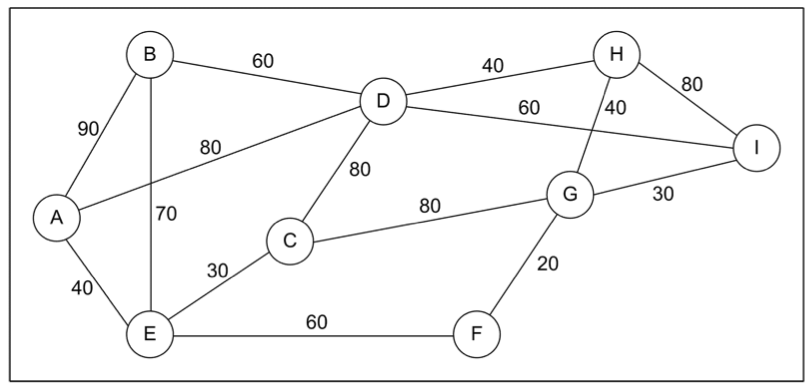
\includegraphics[scale=1]{./img/figure6-24.png}
	\caption{Road network and fuel costs}
	\label{figure6-24}
\end{figure}

\paragraph{(a)}
\begin{quote}
Since this cost is to be incurred every day for a long time, GTC wants to compute the most efficient route to employ in cleaning the area. What is the minimum per day that GTC should be prepared to incur in fuel costs?
\end{quote}

\paragraph{}
We considered a graph with $n=9$ vertices corresponding to points (A, B, \dots, I) and $m=15$ edges corresponding to roads. The weights of the edges are equal to traversing costs. Our problem is equivalent to finding the shortest (minimum total weight) cycle (which may have self-intersections) going through each edge at least once (at least in one direction).

\paragraph{}
To find such path we used the following method. Consider the sought-for optimal cycle. It is also an euler cycle in some supergraph of our graph (with the same verrtices, but with some additional edges). So, the task can be reduced to the following. We need to duplicate some of the edges so that the graph becomes eulerian and the total cost of edges in the graph is minimal. In other words, we need to duplicate some of the edges so that all vertices have even degree.  We can do this using dynamic programming and Dijkstra's algorithm. The state in the DP is a vector of n bits, denoting the parity of degrees of all vertices. The transition of the DP is duplicating some edge: it flips two bits in the bit vector and adds the weight of the edge to the cost. We need to find the shortest path from initial parity vector to zero vector using such transitions. We can use Dijkstra's algorithm for that. Then we can restore the path and duplicate the needed edges. Then we can find euler cycle in the resulting eulerian graph. The algorithm takes $O(2^n n^2 \log n)$ time. This algorithm might seem complicated, but the implementation is concise and much simpler than the implementation of the algorithm with maximum matching of odd-degree vertices.

\paragraph{}
The resulting cheapest round trip going through each road at least once is $ A \rightarrow E \rightarrow F \rightarrow G \rightarrow I \rightarrow H \rightarrow G \rightarrow I \rightarrow D \rightarrow H \rightarrow G \rightarrow C \rightarrow E \rightarrow C \rightarrow D \rightarrow B \rightarrow E \rightarrow A \rightarrow D \rightarrow B \rightarrow A $. It has cost \texteuro 10.6 per day.

\paragraph{(b)}
\begin{quote}
There is some repair work being done on segments between A and D and between G and H. During the time this repair work is on, GTC does not need to wash these segments. The municipality wants to know if GTC would reduce their daily charge, and if so, by how much?
\end{quote}

\paragraph{}
We assume we can still use these two road segments if we like.

\paragraph{}
Now two edges of our graph are not necessary to traverse. In optimal solution each of these two edges is either traversed or not. So, we can try all 4 possibilities of which of these edges are traversed and pick the best solution. If we decide that some edge should not be traversed, we remove it from the graph. Summarizing, the algorithm is as follows: for each of the 4 subsets of two non-necessary edges, remove these edges from the original graph and solve the previous problem on this new graph; choose the best of the 4 answers as final.

\paragraph{}
The new optimal route is $A \rightarrow E \rightarrow F \rightarrow G \rightarrow I \rightarrow H \rightarrow D \rightarrow I \rightarrow G \rightarrow C \rightarrow E \rightarrow B \rightarrow E \rightarrow C \rightarrow D \rightarrow B \rightarrow A$ of cost \texteuro 8.7 per day.

\paragraph{(c)}
\begin{quote}
Consider the situation in part (a). The municipality informs GTC that they are planning a new road between points B and H, and wants GTC to take the responsibility of cleaning this segment at no extra cost. GTC estimates that the fuel cost for traversing this road segment is \texteuro 0.50 per day. Should GTC agree on this extension of contract?
\end{quote}

\paragraph{}
We add the edge B---H of weight 0.5 to the initial graph and solve the same problem as in (a). The resulting optimal route is $A \rightarrow E \rightarrow F \rightarrow G \rightarrow I \rightarrow D \rightarrow I \rightarrow H \rightarrow G \rightarrow C \rightarrow E \rightarrow C \rightarrow D \rightarrow H \rightarrow B \rightarrow E \rightarrow A \rightarrow D \rightarrow B \rightarrow A$ of daily cost \texteuro 10.4. This is \texteuro 0.2 cheaper than in (a), so GTC should gladly agree.

\paragraph{(d)}
\begin{quote}
If the municipality finished constructing the road between B and H while the repair work was being done on segments between A and D and between G and H. If GTC is to take up the road washing activity on the road network including the new road but excluding the segments on which repair work was being done, how much fuel costs would GTC incur per day?
\end{quote}

\paragraph{}
We take the graph from (c) and do with it the same thing as in (b). The resulting route is $A \rightarrow E \rightarrow F \rightarrow G \rightarrow I \rightarrow H \rightarrow G \rightarrow C \rightarrow G \rightarrow I \rightarrow D \rightarrow H \rightarrow B \rightarrow E \rightarrow C \rightarrow D \rightarrow B \rightarrow A$, and the new daily cost is \texteuro 9.4.
